\documentclass[a4paper,norsk,11pt,twoside]{article}
\usepackage[utf8]{inputenc}
\usepackage[T1]{fontenc}
\usepackage[norsk]{babel}
\usepackage{epsfig}
\usepackage{graphicx}
\usepackage{amsmath}
\usepackage{pstricks}
\usepackage{subfigure}
\usepackage{booktabs}       % Pakke for pene tabeller
                            % http://ctan.uib.no/macros/latex/contrib/booktabs/booktabs.pdf

\usepackage[most]{tcolorbox}

\tcbset{
    frame code={}
    center title,
    left=0pt,
    right=0pt,
    top=0pt,
    bottom=0pt,
    colback=gray!70,
    colframe=white,
    width=\dimexpr\textwidth\relax,
    enlarge left by=0mm,
    boxsep=5pt,
    arc=0pt,outer arc=0pt,
    } 

\date{DATO}
\title{AST1100 Prosjekt Del 1}
\author{Daniel Heinesen, daniehei}


% Kommentarer er markert med "%" i margen. Alle disse kan, om du
% ønsker det, fjernes i sin helhet.
% 
% Erstatt ``DOKUMENTTITTEL'' med dokumentets tittel. 
% Erstatt ``FORFATTER'' med ditt navn. 

% Hvis du vil ha dagens dato hver gang du redigerer dokumentet kan du
% bytte ut DATO med \today, ellers erstatter du "DATO" med en fornuftig dato.
 
% Det finnes også ved universitetet en pakke som heter "uioforside", denne kan du lese mer om her. 


\begin{document}
\maketitle
\newpage



\tableofcontents{}

% denne kommandoen gir deg innholdsfortegnelse, såfremt du har brukt \section{} og ikke
% \section*{} (altså at du har valgt nummererte avsnitt).

 

%\section{AVSNITTSOVERSKRIFT}
% 
%% \section{} gir avsnitt
%
%\subsection{UNDER-AVSNITTSOVERSKRIFT}
% 
% % \subsection{} gir under-avsnitt 
%
%
% % Punkt-liste:
%
%\begin{itemize}
%\item{} TEKST
%\end{itemize}
%
%
%
% % Nummerert punktliste:
%
%\begin{enumerate}
%\item{}
%\end{enumerate}
%
%
%
% % Sette inn bilde/figur:
%
%\begin{figure}[hbt]
%\begin{center}
%%\fbox{\includegraphics[width=\textwidth]{}}
%%\caption{BILDEUNDERTEKST}\label{fig:finfigur}}
%\end{center}
%\end{figure} 

\newpage
\part{Motoren}
\newpage

\begin{abstract}
For å starte en romreise, trenger man en motor, og i denne delen skal vi se på hvordan man lager en enkel modell for en slik motor, ved å simulere en boks med partikler. Motoren får fremdriften sin fra bevegelsesmengden av partiklene som går ut gjennom et hull i bunnen av boksen. Vi skal så bruke denne bevegelsesmengden til å regne ut hvor mange slike bokser og hvor mye drivstoff det trengs for å få en rakett ut i verdensrommet.
\end{abstract}

\section{Hvordan lage en motor:}

\begin{abstract}
Målet her er å lage en boks med en haug partikler som spretter rundt i boksen. Vi skal så lage et hull i boksen hvor noen partikler kan forsvinne ut av. Ta av bevegelses mengde i retning nedover, vil gjøre at boksen får en bevegelsenmengde oppover. Dette er grunnprinsippet bak rakettmotoren vår
\end{abstract}

\subsection{Boks med partikler}

\subsubsection{Teori}
Før vi faktisk lager en boks som fungere som en motor, må vi se på en boks uten et hull, og hvordan vi lager trykk i denne. \\

Har man en gass med en temperatur over 0K -- hvilket i praktis alle gasser har -- vil partiklene i denne gassen ha kinetisk energi, som betyr en hastighet. Putter du disse partiklene inn i et lukket rom, vil de kollidere med veggene. Det er disse kollisjonene som gjør at man får et trykk inne i boksen. For å lage motoren vi vil ha på raketten, trenger vi slik en boks med partikler.

\subsubsection{Metode}
Vi starter med én boks med størrelse $L \times L \times L$, hvor $L = 10^{-6} m$. Inne i boksen plasserer vi $N = 10^{5}$ partikler -- nærmere bestemt $H_2$ molekyler -- spredd tilfeldig rundt om i boksen. I tillegg til en posisjon må disse partiklene ha en hastighet. Fra termodynamikken får vi $Maxwell-Boltzmann funksjonen$, som forteller oss fordelingen av hastigheten til partiklene

\begin{equation}
P(\vec{v}) = \left( \frac{m}{2 \pi k T} \right)^{3/2} e^{-\frac{m\vec{v}}{2kT}}
\end{equation}

Vi kan utvidde denne til 

\begin{equation}
P(v_x,v_y,v_z) = \sqrt{\left( \frac{m}{2 \pi k T} \right)} e^{-\frac{m v_x}{2kT}}\sqrt{\left( \frac{m}{2 \pi k T} \right)} e^{-\frac{m v_y}{2kT}}\sqrt{\left( \frac{m}{2 \pi k T} \right)} e^{-\frac{m v_z}{2kT}}
\end{equation}

Hvor $k$ er $Boltzmanns konstant$ og $T$ er temperaturen.
Og siden vi vet at disse er uavhengige sannsyneligheter, så blir

\begin{equation}
P(v_i) = \sqrt{\left( \frac{m}{2 \pi k T} \right)} e^{-\frac{m v_i}{2kT}}
\end{equation}

Det betyr at vi kan vi hver av hastighetskomponentene en tilfeldig fart med en normalfordelig med $\sigma = \sqrt{ \frac{kT}{m}}$
og $\mu = 0$. Partikelens startposisjon i rommet har ikke noe normalfordeling, og plasseres ut med en uniform tilfeldighet.
Vi lar så partiklene snu hastighetskomponenten tilsvarende retningen på normalvektoren til veggen den treffer, m.a.o treffer den høyreveggen snur x-komponenten til partiklen, og tilsvarende for de andre veggene. 

Siden partiklen snur når den treffer en vegg, så må veggen utføre en kraft på den, som kan utrykkes:

\begin{equation}
F_i = \frac{dp}{dt} \approx \frac{\Delta p}{\Delta t} = \frac{2p_i}{\Delta t}
\end{equation}

Dette gir oss så trykket

\begin{equation}
P = \frac{F}{A} = \frac{\frac{2p_i}{\Delta t}}{A} = \frac{2p_i}{\Delta t L^{2}}
\end{equation}

I formelen over er $p_i$ den bevegelsesmengden til alle partiklene som treffer veggen i tidsintervallet $\Delta t$.\\
Ut i fra analytiske utregninger, får vi vite at

\begin{equation}
P = nkT
\end{equation}

hvor $n$ er antall partikler per volum. Dette er en fin måte å sjekke om reultet vi får fra simuleringen er korrekt. Et annet analytisk resultat vi kan sammenlikne med er kinetisk energi. Den analytisk formelen for gjennomsnitts energien til en partikkel er

\begin{equation}
E_k = \frac{3}{2}kT
\end{equation}

Etter vi har kjørt simuleringen sitter vi igjen med men en haug med partikler med en posisjon og en hastighet, fra hastigheten kan vi så regne ut den kinetisk energien

\begin{equation}
E_k = \frac{1}{2n}m_{h2}\sum\limits_{i=1}^{n}(v_x^{2} + v_y^{2} + v_z^{2})
\end{equation}

Så nå har vi satt opp en boks med partikler, i tillegg til to måter vi kan sjekke at vi gjorde det korrekt.

\subsubsection{Utføring og resultater}

I de simuleringene som ble gjort her brukte jeg parameterene at:
\begin{itemize}
\item $T = 10000K$, Temperaturen i kelvin
\item $t = 10^{-9}$, Tidsintervallet jeg brukte i simuleringen
\item $N = 10^{5}$, Antall partikler
\item $Steps = 10000"$, Antall steg i tidsintervallet
\item $\Delta t = t/steps$, Størrelsen på tidsstegene jeg tok
\end{itemize}

For kjøringen av denne simuleringen brukte jeg et smart triks som forenkler kodingen litt: i stedenfor at partiklene beveger seg mellom $0$ og $L$, lar man dem bevege seg mellom $-\frac{L}{2}$ og $\frac{L}{2}$. Dette gjør at når man skal sjekke om de har truffet veggene, så trenger man ikke å sjekke for om $x_i < 0$ eller $x_i > L$, men man trenger bare sjekke om $|x| > L/2$. Men numpy kan dette reduseres til 4 linjer med kode, og kjører raskt. Etter å ha snudd farten plasserer jeg også partiklene på innsiden av veggen. \\

Fra denne simuleringen får jeg:

\begin{tcolorbox}
Analytical Pressure:  13756.1188494 \\
Numerical Pressure:  13800.0 \\
Analytical energy:  2.07e-19 \\
Numerical energy:  2.06623799518e-19 
\end{tcolorbox}

Dette viser at jeg har fått et ganske godt resultat og kan gå videre.

\subsection{En lekkende boks}

\subsubsection{Teori}

Nå som vi har en fungerende boks med partikler, så kan vi prøve å åpne et hull i bunnen. Da vil et vist antall partikler fly ut av hullet. Siden bevegelsesmengden skal være bevart i systemet, og vi mister bevegelsesmengde med partiklene som forsvinner ut gjennom hullet, så må boksen få en like stor, men motsatt rettet bevegelsesmengde. Denne bevegelsesmengden gjør at boksen beveger seg oppover, og vi har en fungerende motor!

\subsubsection{Metode}

Siden vi skal ha en rakettmotor er det naturlig at hullet er i bunnen. Hullet skal også være kvadratisk. Så får å se hvor my kraft vi får i motoren, så teller vi opp bevegelsesmengden partiklene. I tillegg teller vi antallet som forsvinner, siden vi senere vil trenge å vite hvor mye masse som forvinner per tidsenhet. Det er viktig at trykk og temperatur skal holdes konstant hele tiden, dette betyr at vi ikke kan la partiklene som forsvinner ut gjennom hull bli borte, men vi må gjøre noe slik at det alltid er like mange partikler i boksen til en hver tid. Det diskuteres nedenfor hvordan dette gjøres.

\subsubsection{Utføring og resultater}
Jeg bruker alle de samme parameterene som over, men i tillegg bruker jeg at

\begin{itemize}
\item $H = \frac{L}{2}$, Størrelsen på hullet
\end{itemize}

Her kommer det en liten diskusjon om hva man skal gjøre med partiklene som forsvinner gjennom hullet i gulvet. Siden trykket skal holdes konstant, kan man ikke bare la dem forsvinne inn i evigheten. En metode er å plassere dem med en tilfeldig posisjon og hastighet inne i boksen. Dette virker i utgangspunktet som en god metode, men man finner fort ut at trykket og energien vil begynne å synke, dette kan være fordi man gir de partiklene som starter med en stor hastighet nedover en ny tilfeldig fart, mens de som har en lav hastighet for være i fred. M.a.o får man en hopphopning av partikler med lav hastighet. Metoden jeg valgte å gå for var å la disse partiklene som går gjennom hullet bare sprette tilbake -- men telle at de har truffet hullet--. Dette er en urealistisk metode, men bevarer energi og trykk, så derfor valgte jeg å gå får denne.

Det kan være vanskelig å få hullet til å ha rett størrelse, og jeg måtte mange ganger korregere numykoden for å få rett resultat. For å sjekke at riktig mengde partikler gikk gjennom hullet, talte jeg antall partikler som traff gulvet og de som traff hullet. Siden $H = \frac{L}{2}$, så forventer vi at $\frac{1}{4}$ av partiklene som treffer gulvet også går ut gjennom hullet. Jeg valgte også å printe ut informasjon om antall partikler som forsvant per sekund og mengden masse som forsvant per sekund.\\

Sist men ikke har jeg ikke med bevegelsesmengden som boksen fikk, men kraften, da det er den som brukes til alle beregninger videre. \\

Her er resultet


\begin{tcolorbox}
Force:  1.72650965887e-09 \\
Number of particles colliding with floor:  257317 \\
Number of particles escaped:  64252 \\
Number of particles escaped per sec:  6.4252e+13 \\
Mass lost per sec:  2.120316e-13
\end{tcolorbox}

Som vi kan se hadde vi rett, ca $\frac{1}{4}$ av partiklene som traff gulvet forsvant. Men de to tallene vi får bruk for senere er kraften og masse tapt per sekund. Nå som vi har dette, har vi en fungerende motor, og vi kan sende raketen ut i bane



\section{Utregning av drivstoff}

\begin{abstract}
Nå som vi har en motor, og vet hvor mye kraft den gir fra seg og hvor mye masse som forsvinner fra den, kan vi se på hvor mange av disse boksene og hvor mye drivstoff vi trenger, for å sende denne raketten ut i verdensrommet.
\end{abstract}

\subsection{Flere bokser}
Som vi kan se over er kraften fra en boks ikke i nærheten av å få oss noe sted, vi trenger flere bokser -- mange flere. For å finne en brukelig mengde bokser kan vi bruke unnslipshastigheten til planeten som et mål. Denne kan regnes ut ved å finne ut når kinetisk energi er større enn den potensielle energien fra gravitasjonskraften.

\begin{equation}
\frac{1}{2}m v^{2} = \frac{GMm}{r}
\end{equation}

\begin{equation}
v = \sqrt{\frac{2GM}{r}}
\end{equation}

For min planet gir dette at $v \approx 12473 m/s$. Vi kan nå se på et enkelt senario hvor raketten ikke bruker noe drivstoff i oppskytingen velger vi så at raketten skal nå unnslippshastigheten etter 10 min, kan vi regne oss frem til en passende mengde bokser. For å finne mengden bokser bruker vi

\begin{equation}
v(t) = \frac{F}{m} t = \frac{F_{per boks}n_{bokser}}{m_{launcher}} t
\end{equation}

\begin{equation}
n_{bokser} = \frac{v m}{F t}
\end{equation}

Vi får da at vi trenger ca $1.333\cdot 10^{13}$ bokser. Ved å øke tiden vi ønsker å bruke kan vi også senke antallet bokser vi trenger.\\

Vi kan nå bruke dette antallet med bokser, og regne ut hvor mye bensin vi trenger. Vi kan gjøre dette ved å øke farten men akselerasjonen ganger et lite tidssteg, og for vært tidssteg bruker vi "$massen av partiklene som forsvant$" $x tidssteget$ drivstoff. Teller vi hvor mye vi bruker for hvert tidssteg i 10 min, finner vi drivstoffet vi trenger. For min del ble det ca 1696 kg drivstoff -- hvilket passerte testen for drivstoff vi fikk utdelt. Her kan man se en graf av hastigheten og drivstoffet som trengs

\begin{figure}[hbt]
\begin{center}
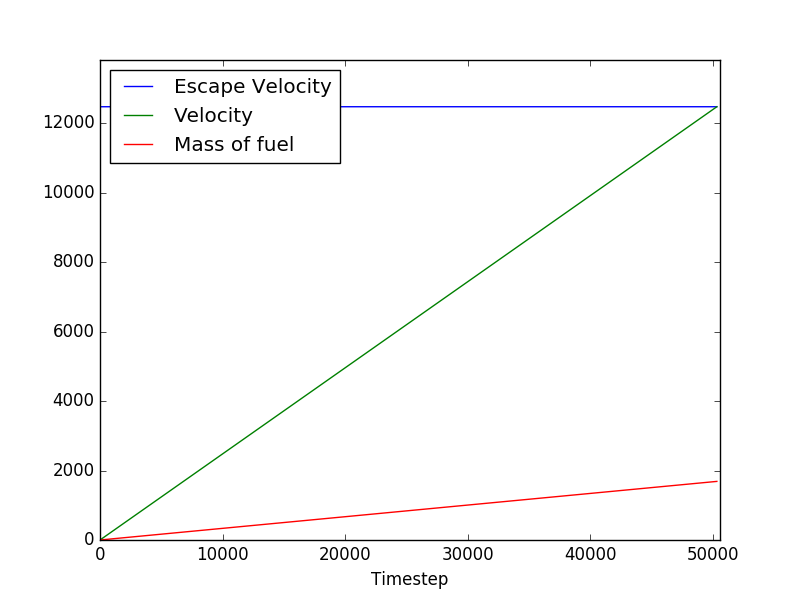
\includegraphics[width=\textwidth]{Fuel_simple.png}
\caption{Simpel drivstoffutregning}\label{fig:finfigur}
\end{center}
\end{figure} 


Siden vi ikke tok med drivstoff når vi beregnet massen, får vi en fin lineær funksjon for hastigheten. \\

Men dette er en urealistisk mengde drivstoff. I en virkelig rakett må man også bære på mass av drivstoffet. I tilegg mister man drivstoff, som gjør at raketten blir lettere, og derfor akselererer raskere jo mer masse som forsvinner. Vi forventer derfor en ikke lineær graf. Her skal vi først bare gjette oss frem til drivstoffet, før vi i neste avsnitt regner oss frem til hvor mye vi trenger. Jeg gjettet ca 4100 kg drivstoff, etter litt prøving og feiling. Vi får da denne grafen:

\begin{figure}[hbt]
\begin{center}
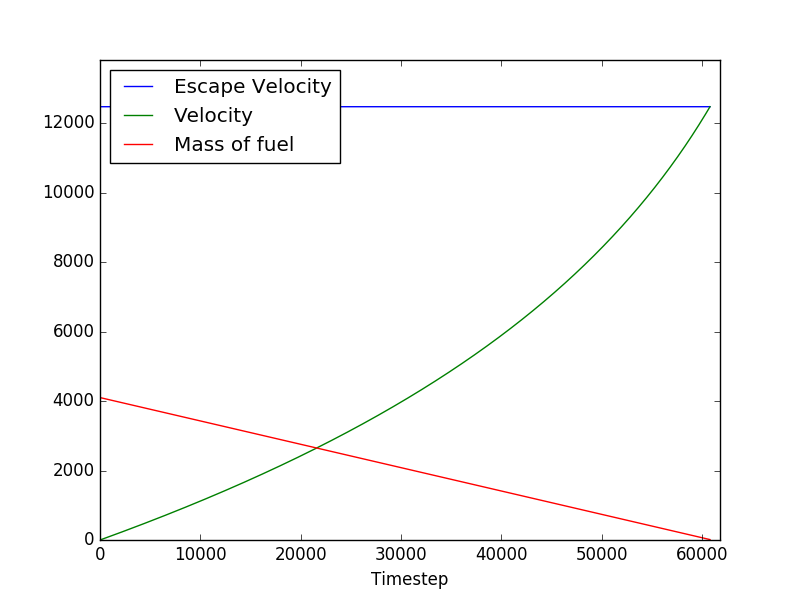
\includegraphics[width=\textwidth]{Fuel_real.png}
\caption{Mer realistisk utregning}\label{fig:finfigur}
\end{center}
\end{figure} 

Med denne gjetningen satt jeg igjen med 12 kg drivstoff, som var ganske nært --jeg jukset litt og brukte formelen jeg regner ut i neste avsnitt. Vi kan også se at stemte antagelsene om hvordan grafen til hastigheten ville se ut. I virkeligheten vil også tyngdekraften spilt en rolle her, og vi ville hatt måtte brukt mye mer drivstoff. \\

Men det er en lang reise vi skal begi oss ut på, så om vi skulle gjettet os frem til riktig mengde drivstoff, ville vi måtte brukt mye tid på prøving of feiling. I stedenfor kan vi regne ut hvor mye vi trenger.


\subsection{Analytisk bereging av drivstoff}

Nå er det på tide å bevege seg litt vekk fra det numerisk og inn i det analytiske, for å finne et begrep som vil gjøre det lettere for oss og bestemme mengden med drivstoff. For å gjøre dette må man ha funnet et antall bokser man vil bruke.Vi starter som man ofte gjør, men Newtons 2. lov:

\begin{equation}
F = ma
\end{equation}

Her må vi bruke det vi fikk fra rakettmotoren som $F$ og $m$, så:

\begin{itemize}
\item $F_b$ er kraften fra hver enkelt boks
\item $n_b$ er antall bokser
\item $m_l$ er massen til laucheren
\item $m_f$ er massen til drivstoffet
\item $m_e$ er massen til partikkelene som går ut av hullet per sekund
\end{itemize}

Da kan vi sette opp en formel for akselerasjon:

\begin{equation}
a = \frac{F}{m} = \frac{F_b n_b}{m_f(t) + m_l} 
\end{equation} 

Og siden massen til drivstoffet endrer seg, må vi skrive dette om til:

\begin{equation}
a = \frac{F_b n_b}{(m_{f0} - n_b n_e t) + m_l} = \frac{F_b n_b}{(m_{f0} - \Delta m t) + m_l}
\end{equation} 

Hvor $\Delta m$ er hvor mye drivstoff som brukes opp hvert sekund.

Vi kan nå gjøre litt fysikkermatte å få at

\begin{equation}
dv = \frac{F_b n_b}{(m_{f0} - \Delta m t) + m_l} dt
\end{equation} 

Så

\begin{equation}
v(t) = \int \frac{F_b n_b}{(m_{f0} - \Delta m t) + m_l} dt
= K - \frac{F_b}{n_e} \ln(m_{tot} - \Delta m t) 
\end{equation}

Der $m_{tot} = m_l + m_{f0}$. Vi kan så sette inn grenseverdien og finne

\begin{equation}
K = v_0 + \frac{F_b}{n_e} \ln (m_{tot})
\end{equation}

Dette gir oss det fine svaret

\begin{equation}
v(t) =v_0 + \frac{F_b}{n_e} \ln \left(\frac{m_{tot}}{m_{tot} - \Delta m t} \right)
\end{equation}

Det vi har kommet frem til nå er rakettlikningen for vår rakett. I den orginale rakettlikningen har vi en konstant som måler effektiviteten til motoren $v_e$, som "den effektive eksoshastigheten". Vi vet nå at denne konstanten er med vår motor gitt som $v_e = \frac{F_b}{n_e}$. (Med litt enkel dimensjonsanalyse finner vi ut at $\frac{F_b}{n_e}$ har de korrekte enhetene)

Men det vi er ute etter er mengden drivstoff vi trenger. For å finne ut dette vil vi at vi sitter igjen uten drivstoff når vi har oppnådd farten vi ville ha. Så med andre ord må $m_{tot} - \Delta m t = m_l$. Med litt algebra får vi da:

\begin{equation}
m_{f0} = m_l(e^{\frac{\Delta v n_e}{F_b}} - 1)
\end{equation}

Vi har nå funnet en enkel formel for å kunne regne ut mengden drivfstoff vi trenger.




 % width = \textwidth gjør at bildet blir like stort som teksten, her kan man endre
 % størrelsen på bildet ved å skrive "width = 10cm" f.eks.

 % "[hbt]" gjør at du prøver å overstyre LaTeX til å putte figuren HER i teksten (h), hvis ikke det går
 % figurer i LaTeX er flytende objekter, og vil gjerne ikke puttes seg akkurat der vi vil...),
 % prøver vi å få LaTeX til å sette figuren på BÅNN av siden (b), hvis ikke det går, så på TOPPEN (t)

 % "\fbox{}" lager en ramme rundt figuren.

 % Latex tar kun .eps-filer (og .ps-filer). Stort sett alle bildeformater kan konverteres til
 % .eps i bildebehandlingsprogrammet Gimp.

 % "\caption" er bildeteksten, hvis du vil ha teksten mindre kan man slenge på "\caption{\small{tekst}}".

 % "\label{}" er figurens "nøkkel". Denne nøklen kan du referere til hvor som helst i teksten din,
 % referansen må da se slik ut: "Se figur \ref{fig:figur1}".

 % Latex må få kompilere to ganger for at den skal få med seg både at det er en referanse,
 % og for å kople referanse og label. 



 % Sette inn formel/matteelement (nummerert):

%\begin{equation}\label{eq:9.141}
%\varrho^{j}_{i}(t) =
%\sqrt{(X^{j}(t)-X_{i}) +(Y^{j}(t)-Y_{i}) +(Z^{j}(t)-Z_{i}) } \equiv f(X_{i}, Y_{i}, Z_{i})
%\end{equation}

 % "\varrho" gir den greske bokstaven rho
 % "\sqrt{}" gir kvadratrot
 % "^{}" betyr at det som står inni {} skal opphøyes, "_{}" betyr det motsatte
 % likningen blir seendes slik ut (står nederst på siden)
 % "\equiv" gir likhetstegn med tre streker
 % equation lager nummererte formler, man kan også bruke "$formel$" hvis man vil
 % ha matteelementer midt i en tekst (altså matteelementer mellom to dollartegn $$). 



 % Sette inn en tabell:

%\begin{table}
%\centering
%\begin{tabular}{c c c c}
%\toprule
%Var1 & Var2 & Var3 & Var4\\
%\midrule
%data & data & data & data\\
%data & data & data & data\\
%\bottomrule
%\end{tabular}
%\caption{TABELLFORKLARINGSTEKST}\label{tab:fintabell}
%\end{table}

 %"|c|c|c|c|" lager en tabell med fire kolonner
 %"\hline" lager en horisontal linje
 %du kan lage så mange rader du vil, hver kolonne i raden skilles med &-tegn.
 % "\caption" og "\label" er det samme som på figur. Man må ikke skrive "{tab:fintabell}",
 % man kan skrive hva man vil, men hvis en skriver et stort dokument kan det være greit å
 % skille mellom referanser som er fra tabeller, likninger, figurer og overskrifter. 





\end{document}